
\documentclass[12pt]{article}
\usepackage{geometry}
\geometry{A4}
\usepackage{graphicx}
\usepackage{amssymb}
\usepackage{amsmath}
\usepackage{algorithm}
\usepackage{algpseudocode}
\usepackage{caption}
\usepackage{indentfirst}
\algnewcommand\algorithmicswitch{\textbf{switch}}
\algnewcommand\algorithmiccase{\textbf{case}}
\algdef{SE}[SWITCH]{Switch}{EndSwitch}[1]{\algorithmicswitch\ #1\ \algorithmicdo}{\algorithmicend\ \algorithmicswitch}%
\algdef{SE}[CASE]{Case}{EndCase}[1]{\algorithmiccase\ #1}{\algorithmicend\ \algorithmiccase}%
\algtext*{EndSwitch}%
\algtext*{EndCase}%

\DeclareCaptionFormat{algor}{%
  \hrulefill\par\offinterlineskip\vskip1pt%
    \textbf{#1#2}#3\offinterlineskip\hrulefill}
\DeclareCaptionStyle{algori}{singlelinecheck=off,format=algor,labelsep=space}
\captionsetup[algorithm]{style=algori}

\usepackage{fontspec,xltxtra,xunicode}
\defaultfontfeatures{Mapping=tex-text}


\title{ICSI403: Assignment 3}
\author{Huang Kaisheng <2020215138@stu.cqupt.edu.cn>}
\date{\today}

\begin{document}
\maketitle
\newpage
\tableofcontents
\newpage

\section{Prob. 1}
Let $h(k) = k \bmod 9$, 
$$
\begin{aligned}
h(5) = 5 \bmod 9 = 5 &,
{\color{blue} h(28) = 28 \bmod 9 = 1} \\
{\color{blue} h(19) = 19 \bmod 9 = 1} &,
{\color{teal} h(15) = 15 \bmod 9 = 6} \\
h(20) = 20 \bmod 9 = 2 &,
{\color{teal} h(33) = 33 \bmod 9 = 6} \\
h(12) = 12 \bmod 9 = 3 &,
h(17) = 17 \bmod 9 = 8 \\
{\color{blue} h(10) &= 10 \bmod 9 = 1}
\end{aligned}
$$

We can see {\color{blue}blue}-marked keys {\color{blue}$28, 19, 10$} are mapped to 1. And {\color{teal}teal}-marked keys {\color{teal}$15, 33$} are mapped to 6. There are two collisions. When we face to a collision, we chain the keys that are mapped to the same hash.

Chained keys: \\
{\texttt{
0 \\
1 -> 28 -> 19 -> 10 \\
2 -> 20 \\
3 -> 12 \\
4 \\
5 -> 5 \\
6 -> 15 -> 33 \\
7 \\
8 -> 17 \\
}
}

\newpage

\section{Prob. 2}

When $m = 1000, A = \frac{\sqrt{5} - 1}{2}$, the hash function $h(k) = \lfloor m(kA \bmod 1) \rfloor = \lfloor 1000(\frac{\sqrt{5} - 1}{2}k \bmod 1) \rfloor$.

For 61, 62, 63, 64 and 65:

$$
\begin{aligned}
h(61)=700 &,
h(62)=318 \\
h(63)=936 &,
h(64)=554 \\
h(65)&=172 \\
\end{aligned}
$$

So they are mapped to 700, 318, 936, 554 and 172.

\section{Prob. 3}
There are $10, 22, 31,4,15, 28, 17, 88,59$ to be inserted.

\subsection{Linear Probing}
Since the size of hash table is 11, actually the hash function $h(k) = k \bmod m = k \bmod 11$.
$$
\begin{aligned}
&h(10)=10 &{} \\
&h(22)=0 &{} \\
&h(31)=9 &{} \\
&h(4)=4 &{} \\
&{\color{cyan}h(15)=4}  &\leftarrow \text{Collision! Insert to next slot 5}  \\
&h(28)=6 \\
&{\color{orange}h(17)=6} &\leftarrow \text{Collision! Insert to next slot 7} \\
&{\color{blue}h(88)=0} &\leftarrow \text{Collision! Insert to next slot 1} \\
&{\color{red}h(59)=4} &\leftarrow \text{Collision! Insert to next slot 6} \\
&{} &\text{but 6 is used, so use the first free slot 8}
\end{aligned}
$$

The finally hash table:

\begin{longtblr}[
  caption = {Hash table with linear probing},
]{
  cell{2}{3} = {fg=blue},
  cell{2}{7} = {fg=cyan},
  cell{2}{9} = {fg=orange},
  cell{2}{10} = {fg=red},
  hlines,
  vlines,
}
Index & 0  & 1  & 2 & 3 & 4 & 5  & 6  & 7  & 8  & 9  & 10 \\
Value & 22 & 88 &   &   & 4 & 15 & 28 & 17 & 59 & 31 & 10 
\end{longtblr}

\subsection{Quadratic Probing with $c_1 = 1$ and $c_2 = 3$}
The hash function $h(k, i) = (h'(k) + c_1 i + c_2 i^2) \bmod m = (k + i + 3i^2) \bmod 11$.

$$
\begin{aligned}
&h(10,0)=10 &{} \\
&h(22,0)=0 &{} \\
&h(31,0)=9 &{} \\
&h(4,0)=4 &{} \\
&{\color{blue}h(15,0)=4} &\leftarrow \text{Collision! } h(15,1)=3\text{, insert to 3} \\
&h(28,0)=6 &{} \\
&{\color{cyan}h(17,0)=6} &\leftarrow \text{Collision! } h(17,1)=5\text{, insert to 5} \\
&{\color{red}h(88,0)=0} &\leftarrow \text{Collision! } h(88,1)=10\text{, but 10 is used.} \\
&{} &{h(88,2)=5\text{,used. }h(88,3)=7, \text{which is a free slot!}} \\
&{\color{orange}h(59,0)=4} &\leftarrow \text{Collision! } h(59,1)=3\text{, but 3 is used.} \\
&{} &{h(59,2)=9\text{,used. }h(59,3)=0\text{,used.}} \\
&{} &{\cdots, h(59,7)=1, \text{which is a free slot!}}
\end{aligned}
$$

The finally hash table:

\begin{longtblr}[
  caption = {Hash table with quadratic probing},
]{
  cell{2}{3} = {fg=orange},
  cell{2}{5} = {fg=blue},
  cell{2}{7} = {fg=cyan},
  cell{2}{10} = {fg=red},
  hlines,
  vlines,
}
Index & 0  & 1  & 2 & 3 & 4 & 5  & 6  & 7  & 8  & 9  & 10 \\
Value & 22 & 59 &   & 15 & 4 & 17 & 28 & 88 & 59 & 31 & 10 
\end{longtblr}

\subsection{Double Hashing with $h_1(k) = k$ and $h_2(k) = 1 + (k \bmod (m – 1))$}
The hash function $h(k, i) = (h_1(k) + ih_2(k)) \bmod m = (k + i(1 + (k \bmod 10)) \bmod 11$.

$$
\begin{aligned}
&h(10,0)=10 &{} \\
&h(22,0)=0 &{} \\
&h(31,0)=9 &{} \\
&h(4,0)=4 &{} \\
&{\color{red}h(15,0)=4} &\leftarrow \text{Collision! } h(15,1)=10\text{, but 10 is used.} \\
&{} &{h(15,2)=5\text{, which is a free slot!}} \\
&h(28,0)=6 &{} \\
&{\color{orange}h(17,0)=6} &\leftarrow \text{Collision! } h(17,1)=3\text{, insert to 3.} \\
&{\color{blue}h(88,0)=0} &\leftarrow \text{Collision! } h(88,1)=9\text{, but 9 is used.} \\
&{} &{h(88,2)=7\text{, which is a free slot!}} \\
&{\color{cyan}h(59,0)=4} &\leftarrow \text{Collision! } h(59,1)=3\text{, but 3 is used.} \\
&{} &{h(59,2)=2\text{, which is a free slot!}}
\end{aligned}
$$

The finally hash table:

\begin{longtblr}[
  caption = {Hash table with double hashing},
]{
  cell{2}{3} = {fg=cyan},
  cell{2}{5} = {fg=orange},
  cell{2}{9} = {fg=blue},
  cell{2}{10} = {fg=red},
  hlines,
  vlines,
}
Index & 0  & 1  & 2 & 3 & 4 & 5  & 6  & 7  & 8  & 9  & 10 \\
Value & 22 & 59 & 15 & 17 & 4 & 15 & 28 & 88 & 59 & 31 & 10 
\end{longtblr}

\newpage
\section{Prob. 4}
$$
\begin{aligned}
&{} &{\{a\}, \{b\}, \{c\}, \{d\}, \{e\}, \{f\}, \{g\}, \{h\}, \{i\}, \{j\}, \{k\}} \\
&{\xrightarrow[\text{iteration }1]{{\color{red}\operatorname{Find-Set}(d) \neq \operatorname{Find-Set}(i)}}} &{\{a\}, \{b\}, \{c\}, \{d, i\}, \{e\}, \{f\}, \{g\}, \{h\}, \{j\}, \{k\}} \\
&{\xrightarrow[\text{iteration }2]{{\color{red}\operatorname{Find-Set}(f) \neq \operatorname{Find-Set}(k)}}} &{\{a\}, \{b\}, \{c\}, \{d, i\}, \{e\}, \{f, k\}, \{g\}, \{h\}, \{j\}} \\
&{\xrightarrow[\text{iteration }3]{{\color{red}\operatorname{Find-Set}(g) \neq \operatorname{Find-Set}(i)}}} &{\{a\}, \{b\}, \{c\}, \{d, g, i\}, \{e\}, \{f, k\}, \{h\}, \{j\}} \\
&{\xrightarrow[\text{iteration }4]{{\color{red}\operatorname{Find-Set}(b) \neq \operatorname{Find-Set}(g)}}} &{\{a\}, \{b, d, g, i\}, \{c\}, \{e\}, \{f, k\}, \{h\}, \{j\}} \\
&{\xrightarrow[\text{iteration }5]{{\color{red}\operatorname{Find-Set}(a) \neq \operatorname{Find-Set}(h)}}} &{\{a, h\}, \{b, d, g, i\}, \{c\}, \{e\}, \{f, k\}, \{j\}} \\
&{\xrightarrow[\text{iteration }6]{{\color{red}\operatorname{Find-Set}(i) \neq \operatorname{Find-Set}(j)}}} &{\{a, h\}, \{b, d, g, i, j\}, \{c\}, \{e\}, \{f, k\}} \\
&{\xrightarrow[\text{iteration }7]{{\color{red}\operatorname{Find-Set}(d) \neq \operatorname{Find-Set}(k)}}} &{\{a, h\}, \{b, d, f, g, i, j, k\}, \{c\}, \{e\}} \\
&{\xrightarrow[\text{iteration }8]{{\color{blue}\operatorname{Find-Set}(b) = \operatorname{Find-Set}(j)}}} &{\{a, h\}, \{b, d, f, g, i, j, k\}, \{c\}, \{e\}} \\
&{\xrightarrow[\text{iteration }9]{{\color{blue}\operatorname{Find-Set}(d) = \operatorname{Find-Set}(f)}}} &{\{a, h\}, \{b, d, f, g, i, j, k\}, \{c\}, \{e\}} \\
&{\xrightarrow[\text{iteration }10]{{\color{blue}\operatorname{Find-Set}(g) = \operatorname{Find-Set}(j)}}} &{\{a, h\}, \{b, d, f, g, i, j, k\}, \{c\}, \{e\}} \\
&{\xrightarrow[\text{iteration }11]{{\color{red}\operatorname{Find-Set}(a) \neq \operatorname{Find-Set}(e)}}} &{\{a, e, h\}, \{b, d, f, g, i, j, k\}, \{c\}} \\
\end{aligned}
$$

\section{Prob. 5}

\subsection{The data structure of the disjoint set $S$}

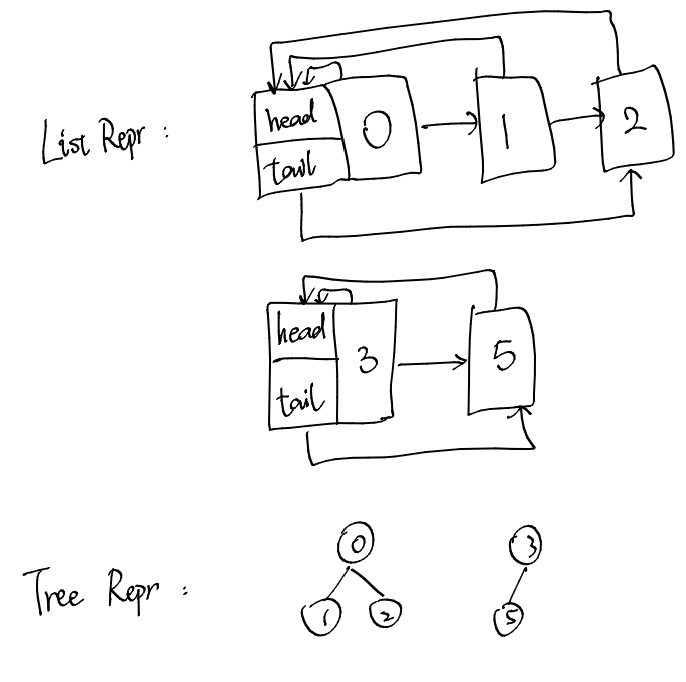
\includegraphics[list representation and tree representation]{pics/as3prob5.1.png}

\subsection{Commands applied to $S$}

\subsubsection{The list representation with weighted union heuristic applied}
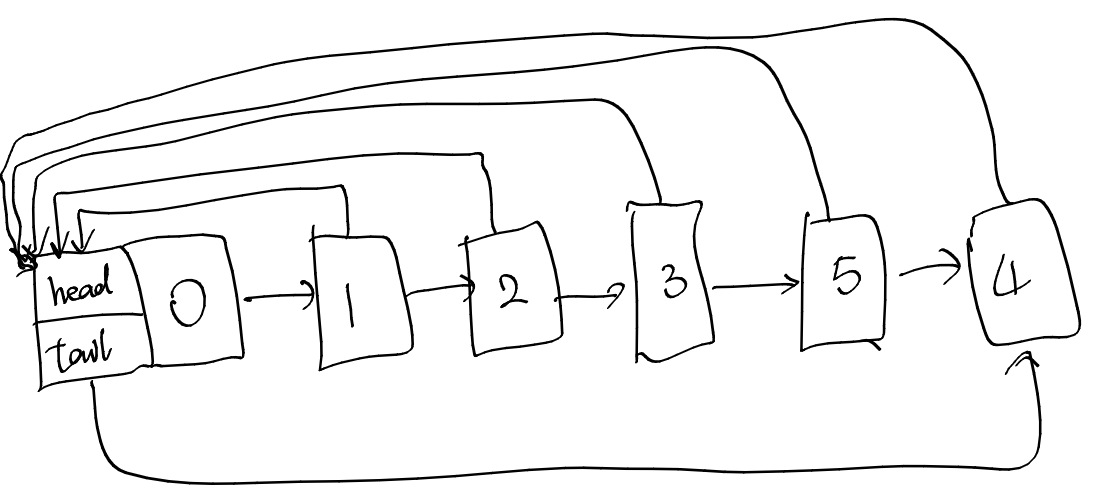
\includegraphics[list representation]{pics/as3prob5.2.png}

\subsubsection{The tree representation with union-by-rank applied}
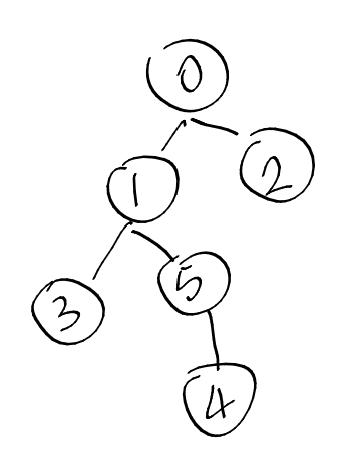
\includegraphics[list representation]{pics/as3prob5.3.png}

\subsection{Path-compression}
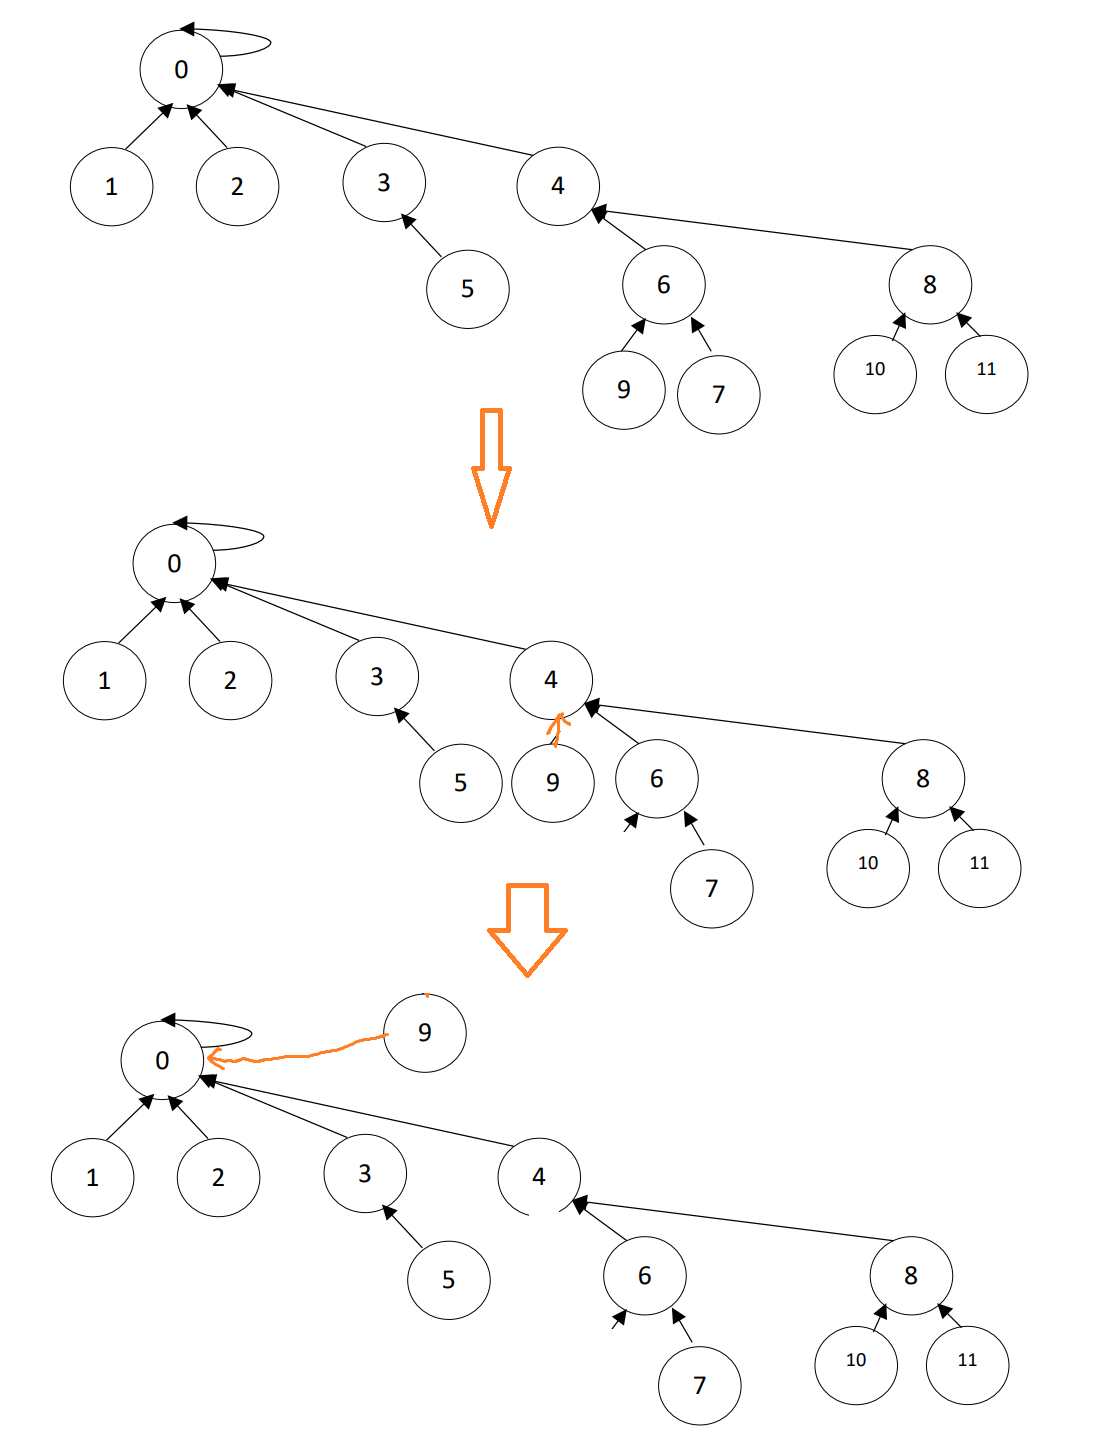
\includegraphics[path compression]{pics/as3prob5.4.png}
\end{document}